%
%===============>>  ГРУППА 5-1 МОДУЛЬ 7  <<=============
%
\setmodule{7}

%BEGIN_FOLD % ====>>_____ Занятие 1 _____<<====
\begin{class}[number=1]
	\begin{listofex}
		\item Выполните действия:
		\begin{tasks}(1)
			\task \( 11,47+(3,89-2,11)-4,416+3,711 \)
			\task \( 3,16+(7,84-4,181)-3,11+14,816 \)
			\task \( 1,49+(6,13-4,12)-0,5+7,289 \)
		\end{tasks}
		\item Вычислите:
		\begin{tasks}(4)
			\task \( 0,5\cdot10 \)
			\task \( 0,15\cdot10000 \)
			\task \( 50,265\cdot10 \)
			\task \( 21,598\cdot1000 \)
			\task \( 9,56\cdot50 \)
			\task \( 8,532\cdot1200 \)
			\task \( 9,123\cdot15000 \)
			\task \( 24,1\cdot130000 \)
		\end{tasks}
		\item Вычислите:
		\begin{tasks}(4)
			\task \( 25,36\cdot1,2 \)
			\task \( 3,5\cdot3,8 \)
			\task \( 63,25\cdot0,3 \)
			\task \( 5,369\cdot0,05 \)
			\task \( 12,03\cdot4,6 \)
			\task \( 23,71\cdot1,8 \)
			\task \( 0,24\cdot5,5 \)
			\task \( 0,7\cdot0,14 \)
		\end{tasks}
		\item Найдите:
		\begin{tasks}(2)
			\task \( 3,5\% \) от \( 1400 \)
			\task \( 12,5\% \) от \( 12500 \)
			\task \( 25,5\% \) от \( 14 \)
			\task \( 0,3\% \) от \( 2 \)
		\end{tasks}
		\item Цену на блузку понизили на \( 11,5\% \). Какой стала её цена, если первоначально она стоила \( 5000 \) рублей?
		\item Максим построил у себя в тетради прямоугольник со сторонами, равными \( 1,8 \) см и \( 5,6 \) см. Найдите периметр и площадь фигуры. Что больше? На сколько?
		\item Костя изобразил треугольник, один угол которого равен \( 23,5\degree \), другой в \( 3,7 \) раза больше. Чему равен третий угол? Чему равны внешние углы этого треугольника?
	\end{listofex}
\end{class}
%END_FOLD

%BEGIN_FOLD % ====>>_____ Занятие 2 _____<<====
\begin{class}[number=2]
	\begin{listofex}
		\item Вычислите 
		\begin{tasks}(4)
			\task \( 1,8\cdot5,5 \)
			\task \( 41,7\cdot6,05 \)
			\task \( 8,42\cdot9,9 \)
			\task \( 6,703\cdot2,45 \)
			\task \( 55,3\cdot3,81 \)
			\task \( 6,321\cdot7,8 \)
			\task \( 32,4\cdot103,5 \)
			\task \( 8,05\cdot8,05 \)
		\end{tasks}
	\item Выполните действия
	\begin{tasks}
		\task \( 4,735\cdot0,5+14,95\cdot1,3+2,121\cdot0,7 \)
		\task \( (0,578+2,172)\cdot(1,823+0,117)-1,711\cdot(0,418+1,382) \)
		\task \( 3,006-0,0417\cdot3-0,875\cdot0,4 \)
	\end{tasks}
	\item Ширина прямоугольника \( 5,15 \) см, а длина в \( 2 \) раза больше. Найдите площадь и периметр данного прямоугольника?
	\item Площадь прямоугольника \( 42 \) см\( ^{2} \), ширина его равна \( 6 \) см. Чему равна длина прямоугольника?
	\item 
	\begin{minipage}[t]{\bodywidth}
		Найдите угол \( \alpha \).
	\end{minipage}
	\hspace{0.02\linewidth}
	\begin{minipage}[t]{\picwidth}
		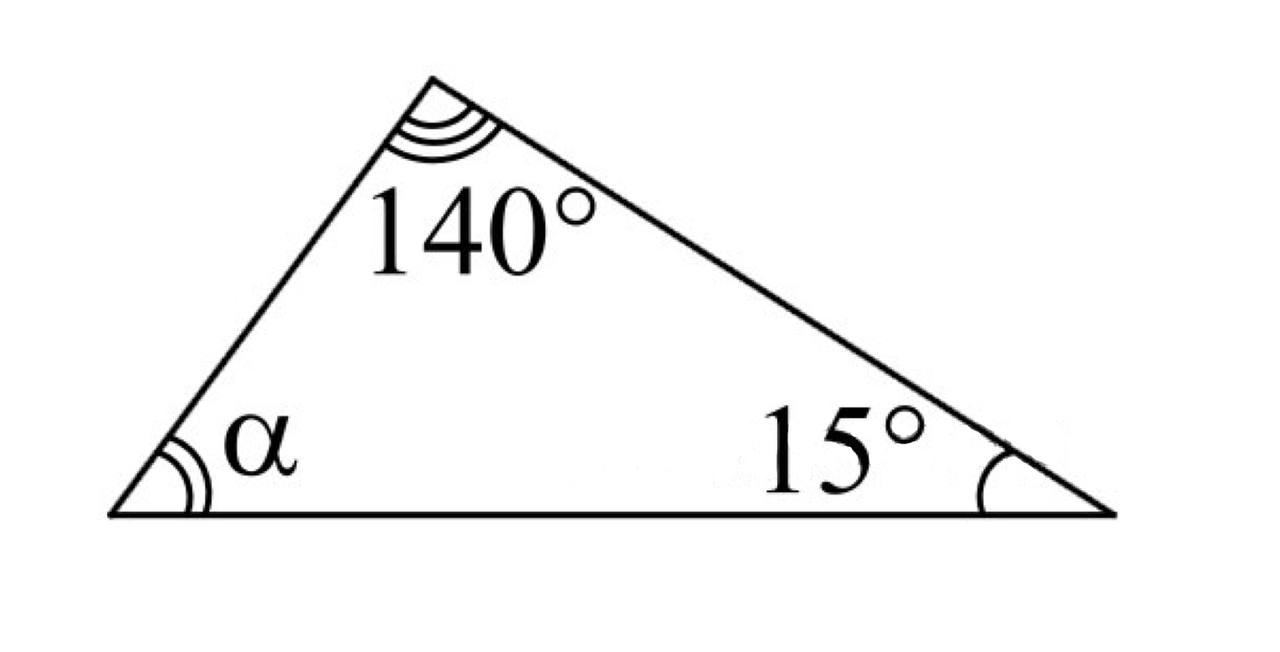
\includegraphics[align=t, width=\linewidth]{\picpath/G51M7L2-1}
	\end{minipage}
	\item 
	\begin{minipage}[t]{\bodywidth}
		Найдите величину угла \( MAB \).
	\end{minipage}
	\hspace{0.02\linewidth}
	\begin{minipage}[t]{\picwidth}
		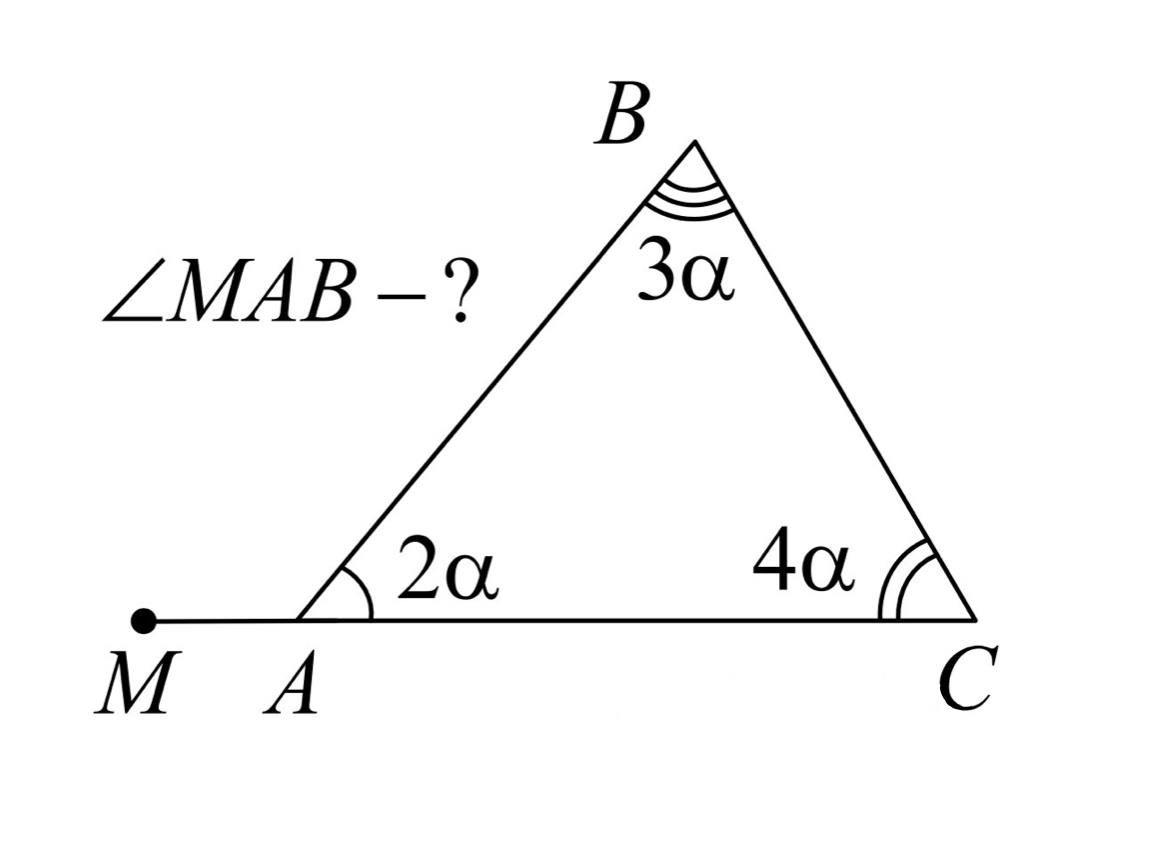
\includegraphics[align=t, width=\linewidth]{\picpath/G51M7L2-2}
	\end{minipage}
	\item Найдите углы треугольника, зная, что внешние углы при двух его вершинах равны \( 130^{\circ} \) и \( 140^{\circ} \).
	\item Один из углов, образовавшихся при пересечении двух прямых, равен \( 45^{\circ} \). Найди остальные углы.
	\item Биссектрисы углов \( N \) и \( M \) треугольника \(  MNP \) пересекаются в точке \( A \). Найдите \( \angle NAM \), если \( \angle N=84^{\circ} \) градусов , а \( \angle M=42 \)градусов . 
	\item Летом на дачу с детским садом собирались поехать \( 180 \) детей. Известно, что \( 15,4\% \) детей не поехали на дачу. Сколько всего детей в детском саду?
	\item Четверть тиража новой газеты раскуплена в первый же день ее выпуска, причем \( 64\% \) этой газеты продано в газетных киосках. Сколько процентов всего тиража продано в газетных киосках?
	\end{listofex}
\end{class}
%END_FOLD

%BEGIN_FOLD % ====>>_ Домашняя работа 1 _<<====
\begin{homework}[number=1]
	\begin{listofex}
		\item Домашняя работа 1
	\end{listofex}
\end{homework}
%END_FOLD

%BEGIN_FOLD % ====>>_____ Занятие 3 _____<<====
\begin{class}[number=3]
	\begin{listofex}
		\item Выполните сложение: \begin{tasks}(3)
			\task \( 0,769 + 42,389; \)
			\task \( 5,8 + 22,191;  \)
			\task \( 95,381 + 3,219; \)
			\task \( 8,9021 + 0,68;  \)
			\task\(  2,7 + 1,35 + 0,8;  \)
			\task\( 13,75 + 8,2 + 0,115. \)
		\end{tasks}
	\end{listofex}
\end{class}
%END_FOLD

%BEGIN_FOLD % ====>>_____ Занятие 4 _____<<====
\begin{class}[number=4]
	\begin{listofex}
		\item Занятие 4
	\end{listofex}
\end{class}
%END_FOLD

%BEGIN_FOLD % ====>>_ Домашняя работа 2 _<<====
\begin{homework}[number=2]
	\begin{listofex}
		\item Домашняя работа 2
	\end{listofex}
\end{homework}
%END_FOLD

%BEGIN_FOLD % ====>>_____ Занятие 5 _____<<====
\begin{class}[number=5]
	\begin{listofex}
		\item Занятие 5
	\end{listofex}
\end{class}
%END_FOLD

%BEGIN_FOLD % ====>>_____ Занятие 6 _____<<====
\begin{class}[number=6]
	\begin{listofex}
		\item Занятие 6
	\end{listofex}
\end{class}
%END_FOLD

%BEGIN_FOLD % ====>>_ Домашняя работа 3 _<<====
\begin{homework}[number=3]
	\begin{listofex}
		\item Домашняя работа 3
	\end{listofex}
\end{homework}
%END_FOLD

%BEGIN_FOLD % ====>>_____ Занятие 7 _____<<====
\begin{class}[number=7]
	\title{Подготовка к проверочной}
	\begin{listofex}
		\item Занятие 7
	\end{listofex}
\end{class}
%END_FOLD

=%BEGIN_FOLD % ====>>_ Проверочная работа _<<====
\begin{exam}
	\begin{listofex}
		\item Проверочная
	\end{listofex}
\end{exam}
%END_FOLD